\documentclass[aps,nofootinbib]{revtex4}
%\documentclass[aps,12pt,nofootinbib]{revtex4}
%\linespread{0.99}

\usepackage{mathpazo}

\usepackage{amsmath}
\usepackage{amsfonts,amssymb,amsthm, bbm,braket}
\usepackage{graphicx}   % need for figures
\usepackage{subfigure}  % and subfigures
\usepackage{amsbsy} % for bold greek letters
\usepackage[bold]{hhtensor} 
\usepackage[all]{xy}

%--------------------------------MACROS-------------------------------------------------------------------------------

\newcommand\red{\color{red}}
\newcommand\magn{\color{magenta}}
\newcommand\Tr{\mathrm{Tr}}

\makeatletter
\newenvironment{chapquote}[2][2em]
  {\setlength{\@tempdima}{#1}%
   \def\chapquote@author{#2}%
   \parshape 1 \@tempdima \dimexpr\textwidth-2\@tempdima\relax%
   \itshape}
  {\par\normalfont\hfill---\ \chapquote@author\hspace*{\@tempdima}\par\bigskip}
\makeatother

\usepackage{textcomp}

%--------------------------------ENVIRONMENTS-------------------------------------------------------------------------------

\newtheorem{definition}{Definition}
\newtheorem{corollary}{Corollary}
\newtheorem{theorem}{Theorem}
\newtheorem{lemma}{Lemma}
\newtheorem{proposition}{Proposition}
\newtheorem{question}{Question}

%--------------------------------ENVIRONMENTS-------------------------------------------------------------------------------

\usepackage[breaklinks=true]{hyperref}

%getting rid of hyperref's ugly boxes.
%From:http://tex.stackexchange.com/a/51349
\hypersetup{
  colorlinks   = true, %Colours links instead of ugly boxes
  urlcolor     = blue, %Colour for external hyperlinks
  linkcolor    = blue, %Colour of internal links
  citecolor   = magenta %Colour of citations
}

\begin{document}

\title{Topological aspect of Chern-Simons quantum field theories}


\author{Ninnat Dangniam}
\affiliation{Center for Quantum Information and Control,University of New Mexico,Albuquerque, New Mexico, 87131-0001}

\begin{abstract}
\end{abstract}

\maketitle

\tableofcontents

%-------------------
\section*{Introduction}
%-------------------

The Chern-Simons theory is a 2+1-dimensional topological field theory developed and linked to knot invariants (no pun intended) in mathematics by Edward Witten in 1989 \cite{Witten89}. The name comes from the fact that its Lagrangian density is proportional to the Chern-Simons form studied by mathematicians Shiing-Shen Chern and James Harris Simons \cite{Chern74}.

In some sense, it is easy to start talking about the Chern-Simons theory by writing the Lagrangian out in full details:
\begin{align*}
\mathcal{L}_{\text CS} = \frac{k}{4\pi} \epsilon^{j k l} (A_j \partial_k A_l + \frac{2}{3} A_j A_k A_l). 
\end{align*}
But underlying this messy index notation is a beautiful geometric picture of gauge theories, explained in Section \ref{geometry}. The Chern-Simons Lagrangian is introduced in Section \ref{chern-simons}. Since the "almost" gauge invariance property and the quantization of the theory involve the path integral formulation of quantum field theory, we only state the results and refer elsewhere for their derivations. Finally, given the connection of the abelian, $U(1)$-Chern-Simons theory to a certain topological invariant, the linking number, we take a look at examples of fractional statistics and topological degeneracy.

%-------------------
\section{Geometry of gauge theories}\label{geometry}
%-------------------
%\begin{chapquote}{C. N. Yang, \emph{Selected Papers, 1945-1980, with Commentary}}
%That non-Abelian gauge fields are conceptually identical to ideas in the beautiful theory of fiber bundles, developed by mathematicians without reference to the physical world, was a great marvel to me. In 1975 I discussed my feelings with Chern, and said "this is both thrilling and puzzling, since you mathematicians dreamed up these concepts out of nowhere." He immediately protested: "No, no. These concepts were not dreamed up. They were natural and real." 
%\end{chapquote}

In gauge theories, there are two basic fields that are effected by gauge transformations: the physical fields (i.e. classical or quantum fields) and the gauge fields. Both can be described in the precise language of differential geometry: they are \emph{sections} of particular kinds of \emph{bundles} over the base spacetime \emph{manifold}. 

The reader might wonder if such abstraction and generality is really needed, but as we shall see, we are interested in phenomena in topological quantum field theories that arise when the base manifold is topologically nontrivial. In essence, we are doing quantum field theories in a curved spacetime, possibly with boundaries and in dimension other than $3+1$. 

To develop this language as used by mathematicians would require a book or two. Indeed, the development in this section and the discussion of holonomy in the next section follows the delightful book by John Baez and Javier P. Muniain, \emph{Gauge Fields, Knots, and Gravity} \cite{Baez94}. But I believe that we already have a good enough geometrical intuition of many notions in differential geometry that would otherwise require and pages of definitions and theorems to justify rigorously. Two of these notions to start with are that of a manifold and a tangent space. 

%-------------------
\subsection{Manifolds and tangent spaces}
%-------------------

A (smooth) {\bf manifold} $M$ is a space that looks locally Euclidean and  on which we can do calculus. A manifold is covered by a collection of Euclidean patches called chart. Formally, a {\bf chart} $\phi_{\alpha}$ is a map from an open set $U_{\alpha}$ to $\mathbb{R}^d$, where $d$ is the dimension of the manifold, roughly the number of parameters required to parametrize it. So we can do a computation in a chart exactly like how we do it in $\mathbb{R}^d$.
\begin{center}
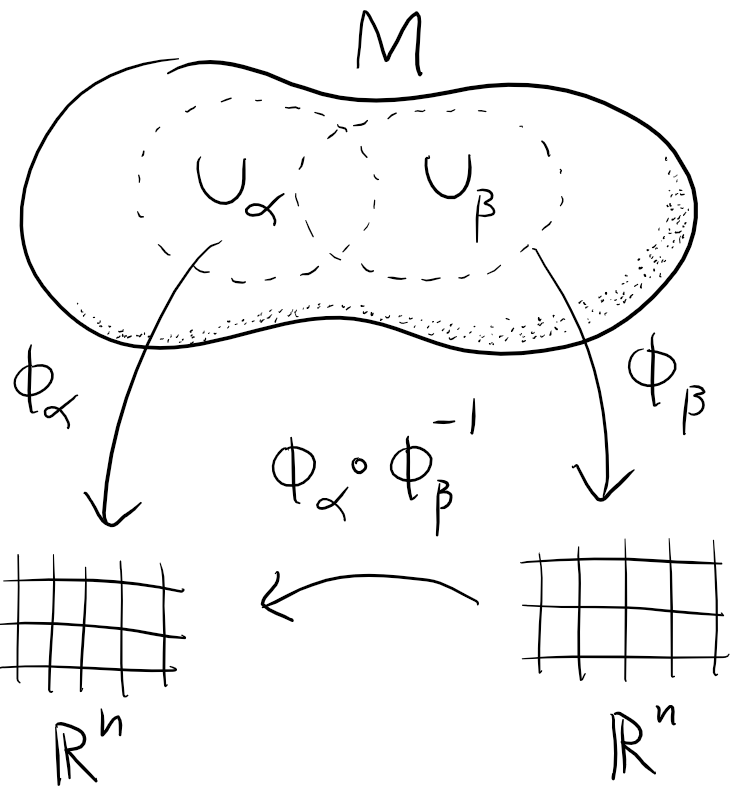
\includegraphics[width=0.3\textwidth]{manifold.png}
\end{center}
We also require that the transition function between overlapping charts $U_{\alpha} \cap U_{\beta}$
\begin{align*}
\phi_{\alpha \beta} = \phi_{\alpha} \circ \phi_{\beta}^{-1}
\end{align*}
is infinitely differentiable, that is, a function in $C^{\infty}$ so that a smooth object in one chart remains smooth in all other overlapping charts. This local chart is required because in general a manifold cannot be covered by just a single chart, just as the globe cannot be represented faithfully by a 2-dimensional map.

The {\bf tangent space} $T_p M$ at point $p$ in an $n$-dimensional manifold $M$ is an $n$-dimensional vector space of {\bf tangent vectors}, all possible directions emanated from $p$. For a flat manifold $M = \mathbb{R}^d$, the manifold and the tangent space are isomorphic and we do not distinguish them. But evoking the sphere as an example again, a tangent vector needs not lie in the manifold in general.
\begin{center}
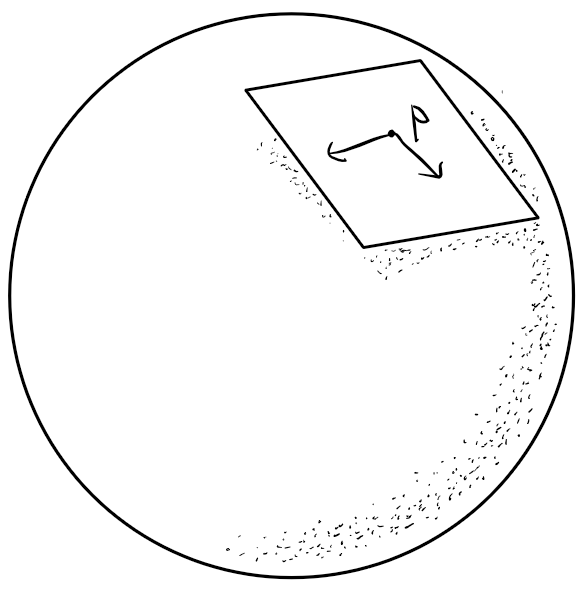
\includegraphics[width=0.3\textwidth]{tangent.png}
\end{center}

%-------------------
\subsection{Vector bundles}
%-------------------

We have said that the sections of particular bundles over a manifold play the role of fields in gauge theories. Consider first a concrete example of a bundle: the {\bf tangent bundle} $TM$ over an $n$-dimensional manifold $M$. It is the collection of tangent spaces at every point $p \in M$.
\begin{align*}
TM &= \bigcup_{p \in M} T_p M.
\end{align*}
Thus a point in $TM$ is a pair $(p,v)$ of a point $p \in M$ and a tangent vector $v$ at that point. So $TM$ is a manifold of dimension $2n$. There is always a surjective projection $\pi$ from the bundle to $M$, sending $(p,v)$ to $p$. So a tangent bundle can be specified as $\pi:TM \to M$.

In a more general bundle
\begin{align*}
\pi: E \to M,
\end{align*}
the manifold $E$ is called the {\bf total space}, the manifold $M$ is called the {\bf base space}, and $\pi$ is still a surjective projection from $E$ to $M$. The pre-image $\pi^{-1}(p)$ is called the {\bf fiber} at $p$. The fiber $E_p$ now does not have to be a tangent space, but we are still interested in the case when the fiber bundle is a vector space. From this point on, every bundle will be such a bundle, called a {\bf vector bundle}. A right inverse of the projection
\begin{align*}
\sigma : M &\to TM \\
	\pi \circ \sigma &= 1,
\end{align*}
where 1 is the identity map, is called a {\bf section} of the bundle. It assigns to each point in the base space a vector in $E_p$. For the tangent bundle, a section is nothing more than a {\bf vector field}. But as we alluded to, the physical fields and the gauge fields will be sections of a more general vector bundle. 
\\ \\ 
{\bf Example.} Gauge fields will turn out to be sections of an {\bf endomorphism bundle} End$(E)$ of $E$. It is the bundle with the same base space $M$ as $E$ but with End$(E)$, the vector space of all linear transformations from $E_p$ to itself, as a fiber at every $p \in M$. \\ 

%The space of all sections $\Gamma (E)$ is a $C^{\infty} (M)$-module, where $C^{\infty} (M)$ is viewed as a ring of smooth functions --- the smooth algebra. 

A bundle $E$ is {\bf trivial} if it is just a Cartesian product $E = M \times F$, where $F$ is called a {\bf standard fiber}.
\begin{figure}
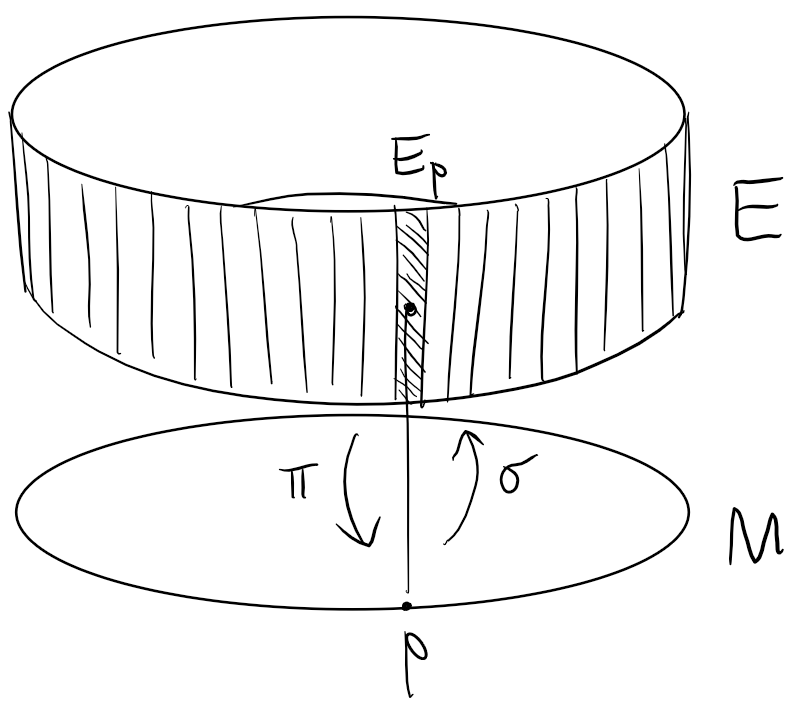
\includegraphics[width=0.35\textwidth]{fiber_bundle.png}
\caption{A cylinder is a trivial fiber bundle with a circle as the base manifold.}
\end{figure}
Trivial bundles are not so interesting. Nevertheless every bundle that we come across will be {\bf locally trivial}. Local triviality with respect to the standard fiber $F$ means that there exists a neighborhood $U$ of each point $p \in M$ and a bundle isomorphism
\begin{align*}
\phi: E\big|_U \to U \times F,
\end{align*}
sending each fiber to the trivial bundle $U \times F$. That is to say, $E$ is locally indistinguishable from the trivial bundle.

Going in reverse, a nontrivial bundle can be built up by gluing trivial bundles together. In a {\bf $G$-bundle} \footnote{In some terminology, a $G$-bundle or a principal $G$-bundle is not a vector bundle, but its associated vector bundle is. What we describe is the associated vector bundle.}, the transition function between overlapping neighborhoods $U_{\alpha} \cap U_{\beta}$ in $M$:
\begin{align*} 
\phi_{\alpha \beta} &= \phi_{\alpha} \circ \phi_{\beta}^{-1}
\end{align*}
where $\phi_{\alpha}: E\big|_{U_{\alpha}} \to U_{\alpha} \times F$ must be an element of the {\bf gauge group} G. (The idea of the transition function between local trivial bundles is analogous to that between charts on a manifold.) The fiber $F$ at each point is now a vector space $V$ on which $G$ acts with a representation $\rho$.
\begin{figure}
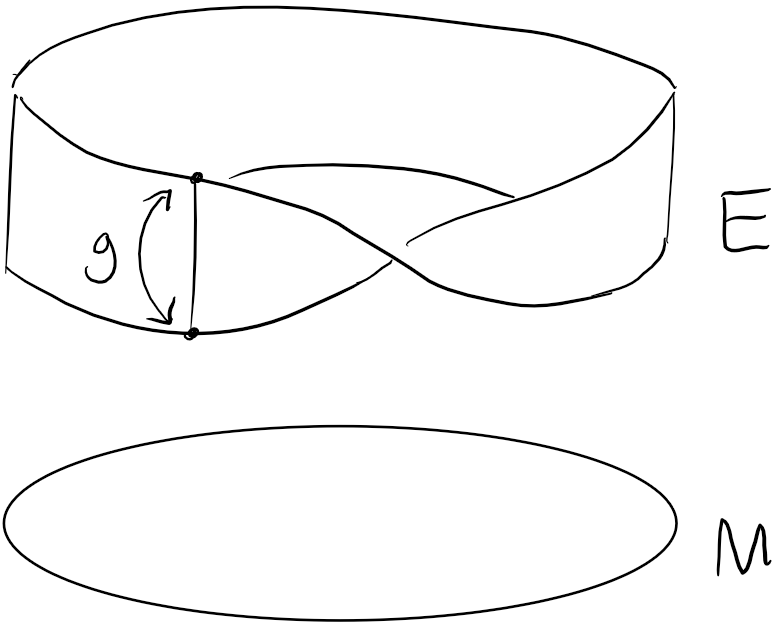
\includegraphics[width=0.35\textwidth]{mobius.png}
\caption{A m{\"o}bius strip has the same base manifold as the cylinder but is not a trivial bundle thanks to the twist $g\in \mathbb{Z}_2$ that joins the opposite ends of the fibers.}
\end{figure}
Simultaneous actions of $G$ on every fiber with the same element $g$ are called {\bf global gauge transformations}, whereas simultaneous actions of $G$ with $g$ that depends on each point in the manifold are {\bf local gauge transformations}.

We can finally state the philosophy of gauge theories. In a gauge theory, the physical field is a section of a $G$-bundle for some group $G$ and if a section $s$ is a solution to the equation of motion (the "physical law"), then $gs$ is also a solution for any local gauge transformation $g$.

%-------------------
\subsection{Connections and gauge fields}
%-------------------
To ensure that the equation of motion is gauge-invariant, it suffices to make the action gauge-invariant. This can be done by "gauging": replacing ordinary derivatives with {\bf connections} (or covariant derivatives). The name comes from the fact that a connection allows us to compare sections at two different points in the manifold and hence allows us to differentiate a section.  (Connections also play a central role in the concept of parallel transport, which will be discussed in Section \ref{Wilson}.)

A {\bf connection} $\nabla$ on a general vector bundle satisfies the following axioms: Given a function $f \in C^{\infty} (M)$, tangent vectors (a direction) $\mu,\nu$ at a point $p \in M$ and a section $s$, a connection is
\begin{enumerate}
\item $C^{\infty} (M)$-linear in $\mu$
\begin{align}
\nabla_{f\mu + \nu} s = f \nabla_{\mu} s + \nabla_{\nu} s,
\end{align}
\item Additive in $s$
\begin{align}
\nabla_{\mu} (s+t) = \nabla_{\mu} s + \nabla_{\mu} t,
\end{align}
\item And obeys the Leibniz law
\begin{align}
\nabla_{\mu} (fs) = (\partial_{\mu} f) s + f \nabla_{\mu} s. 
\end{align}
\end{enumerate}
This is quite abstract, so let us express a connection in coordinates. With the help of a local basis of section $\{e_{\mu}\}$, every section $s$ can be written as $s = s^{\mu} e_{\mu}$. Then the connection of $s$ along the coordinate $\nu$ is 
\begin{align*}
\nabla_{\nu} s &= \nabla_{\nu} (s^{\mu} e_{\mu}) \\
	&= (\partial_{\nu} s^{\mu}) e_{\mu} + A^{\rho}{}_{\nu \mu} s^{\mu} e_{\rho} \\
    &= (\partial_{\nu} s^{\mu} + A^{\mu}{}_{\nu \rho} s^{\rho})e_{\mu},
\end{align*}
\begin{align}
\boxed{ \nabla_{\nu} = \partial_{\nu} s^{\mu} + A^{\mu}{}_{\nu \rho} s^{\rho}}
\end{align}
where we write $A^{\rho}{}_{\nu \mu} e_{\rho} = \nabla_{\nu} e_{\mu}$ and we have only used the Leibniz law. Thus, $A$ specifies how we twist the basis section when we move from one point to another.
If the indices $\mu$ and $\rho$ are fixed, $A$ is an {\bf endomorphism-valued 1-form} over $E$ or an {\bf End$(E)$-valued 1-form}. We will say more about forms and operations on them in the next subsection, but for now it means that upon receiving a vector along a coordinate $\nu$, $A_{\nu}$ gives a linear transformation on the fiber $E_p$. So $A$ itself is also a section, not of $E$ but of End$(E)$.

In a $G$-bundle, $A$ is called a {\bf gauge field} \footnote{For this reason, the gauge field is the same kind of object as the Christoffel symbol in general relativity.} and it is also effected by gauge transformations. Suppose that a section $s$ is transformed to $gs$. There is a new connection $\nabla'$ such that
\begin{align*}
\nabla_{\mu}' (gs) &= g\nabla_{\mu} s \\
\nabla_{\mu}' (s) &= g\nabla_{u} (g^{-1} s) \\
\partial_{\mu} s + A'^{\mu}{}_{\nu \rho} s^{\rho} e_{\mu} &= g \left( \partial_{\mu} g^{-1} s + A^{\mu}{}_{\nu \rho} g^{-1} s^{\rho} e_{\mu} \right) \\
	&= \left( g A_{\mu} g^{-1} \right) (s) + g (\partial_{\mu} g^{-1}) s + \partial_{\mu} s.
\end{align*}
Canceling the $\partial_{\mu} s$ from both sides, we obtain the formula for a gauge transformation
\begin{align}
\boxed{A'_{\mu} = g A_{\mu} g^{-1} + g \partial_{\mu} g^{-1}}.
\end{align}
Observe that a derivative of a Lie group elements is a Lie algebra element. So locally the connection 1-form can also be thought of as a {\bf Lie algebra-valued 1-form} or {\bf $\mathfrak{g}$-valued 1-form} over the $G$-bundle. \\ \\ 
{\bf Example.} When $G$ is abelian, $A$ is just a number and hence commutes with $g$, reducing the formula to
\begin{align}
A'_{\mu} = A_{\mu} + g \partial_{\mu} g^{-1}.
\end{align}
QED is an example of abelian gauge theory with $U(1)$ gauge group. Every element of $U(1)$ can be written as $g = e^{-if}$ for some real function $f$. So the gauge transformation of the potential is
\begin{align}
A_{\mu}' = A_{\mu} + i \partial_{\mu} f.
\end{align}
The new potential differs by a derivative of a function times $i$. This can be made to agree with what we learned in classical electromagnetism simply by replacing $A$ in the connection with $iA$.

%-------------------
\subsection{Differential forms}
%-------------------

We generalize a bunch of things we know from calculus in 3 dimensions.

The dual space $V^*$ of a vector space $V$ over a field $k$ is the space of all linear functionals that act on a vector to produce a number:
\begin{align*}
\omega: V \to k,
\end{align*}
a {\bf 1-form}. This generalizes the idea of inner product. If $V$ has an inner product "$\cdot$", then there is a vector $w \in V$ such that
\begin{align*}
\omega (v) = w \cdot v.
\end{align*}
Therefore $V$ and $V^*$ can be identified. ($V^*$ has the same dimension as $V$.) But there is no canonical choice of an inner product.

The {\bf wedge product} $\wedge$ on a vector space $V$ generalizes the idea of the cross product. In particular, it is bilinear, associative, and antisymmetric
\begin{align}
u \wedge v = - v \wedge u,
\end{align}
where $u,v \in V$. The antisymmetry means that the wedge product of linearly dependent vectors always vanishes. So we can have at most an $n$-fold product of vectors in $V$ if $V$ has dimension $n$. If the vector space of all $p$-fold product of vectors is denoted by $\Lambda^p V$, the {\bf exterior algebra} $\Lambda V$ generated by the wedge product on $V$ is graded by $p$ --- the degree.
\begin{align*}
\Lambda V = \bigoplus_{p=1}^n \Lambda^p V
\end{align*}
If elements of $V$ are 1-forms, we say that elements of $\Lambda^p V$ are {\bf p-forms}.

An aside: the definition of $p$-forms by the antisymmetry property still does not quite say what they are explicitly. Another way to think about them is that they are fully antisymmetric tensors on $V^{\otimes p}$ constructed by antisymmetrization $\mathcal{A}$
\begin{align}
u_1 \wedge u_2 \wedge \cdots \wedge u_n = \mathcal{A} [u_1 \otimes u_2 \otimes \cdots \otimes u_n] 	
	&= \frac{1}{n!} \sum_{\sigma \in S_n} (-1)^{{\text sgn} \sigma} u_{\sigma(1)} \otimes u_{\sigma(2)} \otimes \cdots \otimes u_{\sigma(n)},
\end{align}
where $\sigma$ is a permutation in the symmetric group $S_n$ and sgn $\sigma$ is 1 for an odd permutation and 0 for an even permutation. In the index notation, there is a shorthand using the Levi-Civita symbol
\begin{align}
\mathcal{A} \left[ T_{j_1,j_1,\dots,j_n} \right] &= \frac{1}{n!} \epsilon^{j_1,j_1,\dots,j_n} T_{j_1,j_1,\dots,j_n}.
\end{align}

To motivate the notion of differential forms, consider the gradient $\nabla f$ of a function $f$ in 3 dimensions. ($\nabla$ here is not a general connection.) The gradient should be thought of as a 1-form for the following reason: It acts linearly on a vector and produces a number: the directional derivative
\begin{align}
\nabla f \cdot e_{\mu} = \partial_{\mu} f.
\end{align}
But more than that, we can have a directional derivative along a vector field $s$ because the gradient is also a $C^{\infty}(M)$-linear functional. (Recall that a vector field is a section of the tangent bundle, and the space of all sections $\Gamma(E)$ is a $C^{\infty} (M)$-module, where a module is like a vector space except that the "scalars" can be elements in an arbitrary ring. In this case, it is the ring of $C^{\infty}$ function on $M$.) That is, for any smooth function $g$,
\begin{align}
\nabla f \cdot (g s) = g (\partial_{\mu} s).
\end{align}
We call such a $C^{\infty}(M)$-linear functional a {\bf differential 1-form}. All {\bf differential forms} on $M$ can then be generated by the same construction used to generate the exterior algebra.
\begin{align*}
\Omega (M) = \bigoplus_{p=1}^n \Omega^p (M)
\end{align*}   
This leads to the idea of the {\bf exterior derivative} $d$ that turns a function $f$ (thought of as a differential 0-form) into a differential 1-form $df$ or more generally, turns a differential $p$-form into a differential $p+1$ form. The exterior derivative is defined by the following axioms:
\begin{enumerate}
\item $df$ is a differential 1-form $df = f_{\mu} dx^{\mu}$, where the coordinate 1-forms $dx^{\mu}$ is defined by $dx^{\mu} (x_{\nu}) = \delta^{\mu}{}_{\nu}$
\item $d$ is scalar-linear.
\item $d(\omega \wedge \mu) = d\omega \wedge \mu - (-1)^{p} \omega \wedge d\mu $ when $\omega \in \Omega^p (M)$.
\item $d(d\omega) = 0$ for any $\omega \in \Omega(M)$
\end{enumerate}
These are again quite abstract, but they do capture not only the gradient, but also the divergence and the curl and the relation between them in 3 dimensions. These are worked out in Appendix \ref{appendix}. \\ \\
{\bf Example.} In coordinates, the connection 1-form is
\begin{align}
A &=  A^{\mu}{}_{\nu \rho} e_{\mu} \otimes dx^{\rho} \otimes dx^{\nu},
\end{align} \\
The {\bf curvature} is an antisymmetric 2-form
\begin{align}
F(\mu ,\nu) \equiv \nabla_{\mu} \nabla_{\nu} - \nabla_{\nu} \nabla_{\mu} - \nabla_{[\mu ,\nu]},
\end{align}
where $[\mu ,\nu]$ in coordinates is the direction of the mixed partial derivatives $\partial_{\mu} \partial_{\nu} - \partial_{\nu} \partial_{\mu}$. It measures the failure of the derivatives $\nabla_{\mu}$ and $\nabla_{\nu}$ to commute. The last term corrects for the noncommutativity that arises from the choice of coordinates itself.
\begin{center}
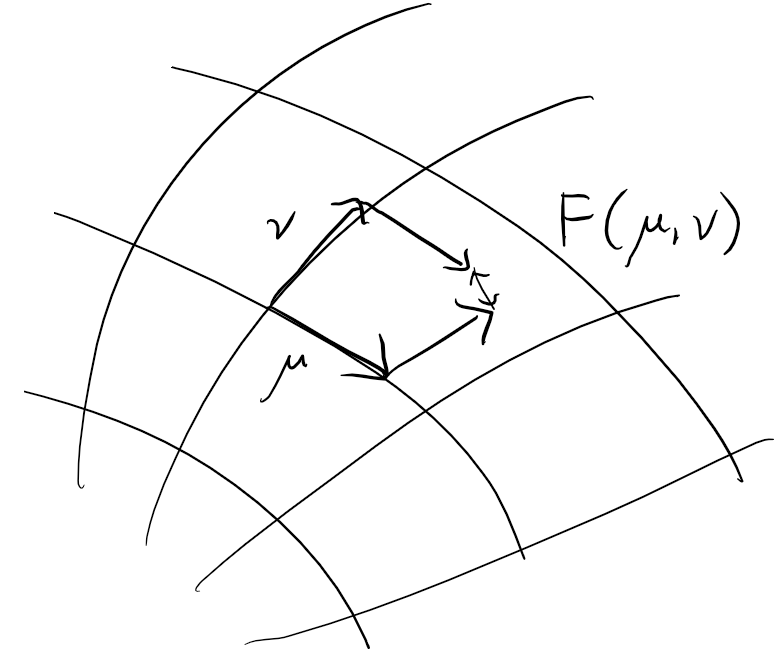
\includegraphics[width=0.3\textwidth]{curvature.png}
\end{center}
To write the curvature in coordinates, let us pick the so-called holonomic basis $\{e_{\mu}\}$ where we do not have the last term. Then
\begin{align*}
F_{\mu \nu} e_{\rho} &= \nabla_{\mu} \nabla_{\nu} e_{\rho} - \nabla_{\nu} \nabla_{\mu} e_{\rho} \\
	&= \nabla_{\mu} ( A^{\xi}{}_{\nu \rho} e_{\xi}) - \nabla_{\nu} (A^{\xi}{}_{\mu \rho} e_{\xi}) \\
    &= (\partial_{\mu} A^{\xi}{}_{\nu \rho}) e_{\xi} + A^{\eta}{}_{\mu \xi} A^{\xi}_{\nu \rho} e_{\eta} - 
    (\partial_{\nu} A^{\xi}{}_{\mu \rho}) e_{\xi} - A^{\eta}{}_{\nu \xi} A^{\xi}_{\mu \rho} e_{\eta} \\
    &= \left( \partial_{\mu} A^{\xi}_{\nu \rho} - \partial_{\nu} A^{\xi}{}_{\mu \rho} + A^{\xi}{}_{\mu \eta} A^{\eta}{}_{\nu \rho} - A^{\xi}{}_{\nu \eta} A^{\eta}{}_{\mu \rho} \right) e_{\xi}
\end{align*}
Suppressing the first and third indices of $A$ that are waiting for contraction, we get
\begin{align}
\boxed{F_{\mu \nu} = \partial_{\mu} A_{\nu} - \partial_{\nu} A_{\mu} + [A_{\mu},A_{\nu}]}.
\end{align}
The commutator does not vanish in general due to the fact that $A_{\mu}$ are matrices. It does not vanish, for instance, when the gauge group $G$ is non-abelian. (Recall that $A$ is a Lie algebra-valued 1-form.) The curvature 2-form clearly generalizes the electromagnetic tensor.

We can also see from
\begin{align}
F = \frac{1}{2} F_{\mu \nu} dx^{\mu} \otimes dx^{\nu},
\end{align}
that the coordinate-free expression of the curvature 2-form is
\begin{align}\label{curvature 2-form}
\boxed{ F = dA + A \wedge A }.
\end{align}

Before we end this section, it will prove necessary to know some algebra of $p$-forms. The wedge product is antisymmetric for 1-forms (but not End$(E)$-valued 1-form!) but for $p$- and $q$-forms,
\begin{align}\label{graded commutative}
\omega \wedge \mu = (-1)^{pq} \mu \wedge \omega.
\end{align}
An End$(E)$-valued $p$-form $S \otimes \omega$ has both the matrix part $S$ and the form part $\omega$. The wedge of product of two End$(E)$-valued forms can be defined as
\begin{align}
(S \otimes \omega) \wedge (T \otimes \mu) \equiv ST \otimes (\omega \wedge \nu),
\end{align}
where $ST$ is the usual matrix product. The trace of an End$(E)$-valued form is the trace of the matrix part
\begin{align}
\Tr (S \otimes \omega) \equiv \Tr (S) \omega.
\end{align}
and the exterior derivative operates on the form part
\begin{align}
d \Tr (S \otimes \omega) = \Tr (S \otimes d\omega).
\end{align}
From \eqref{graded commutative},
\begin{align}
\Tr (S \otimes \omega \wedge T \otimes \mu) &= (-1)^{pq} \Tr (ST) (\mu \wedge \omega) \nonumber \\
	&= (-1)^{pq} \Tr(TS) \otimes (\mu \wedge \omega) \nonumber \\
    &= (-1)^{pq} \Tr (T \otimes \mu \wedge S \otimes \omega). \label{graded cyclic}
\end{align}
As a result, for any End$(E)$-value 1-form $A$,
\begin{align}
\Tr (A \wedge A) &= \frac{1}{2} \Tr ([A,A]) = 0
\end{align}
and
\begin{align}\label{trace of A^4}
\Tr (A \wedge A \wedge A \wedge A) = 0.
\end{align}

%-------------------
\section{Chern-Simons theories}\label{chern-simons}
%-------------------
%\begin{chapquote}{John Preskill, \href{https://quantumfrontiers.com/2015/08/09/kitaev-moore-read-share-dirac-medal/}{a Quantum Frontiers blog post}}
%Anyon, anyon, where do you roam? \\ Braid for a while before you go home. \\ \\ Though you\textquotesingle re condemned just to slide on a table, \\ A life in 2D also means that you\textquotesingle re able \\ To be of a type neither Fermi nor Bose \\ And to know left from right --- that\textquotesingle s a kick, I suppose.
%\end{chapquote}

We are all familiar with the source-free electromagnetic Lagrangian density
\begin{align*}
\mathcal{L}_{\text EM} (A_{\mu}) = -\frac{1}{4} F_{\mu \nu} F^{\mu \nu}, 
\end{align*}
where $F_{\mu \nu} = \partial_{\mu} A_{\nu} - \partial_{\nu} A_{\mu}$. This Lagrangian is not amenable to the coordinate-free formulation with the tools that we have so far since it relies on a metric, and we have not said anything about a metric, for a good reason! Consider instead the somewhat similar-looking but metric-free {\bf 2nd Chern form}
\begin{align*}
\Tr (F \wedge F).
\end{align*}
It turns out that, the action of this Lagrangian is extremized for all choices of $A$ by the Bianchi identity \cite{Baez94} so it gives a rather boring physical theory. But if we  instead expand it in terms of the connection 1-form $A$ and use \eqref{graded commutative} and \eqref{trace of A^4}, we find that
\begin{align*}
\Tr (F \wedge F) &= \Tr \left[ (dA + A \wedge A) \wedge (dA + A \wedge A) \right] \\
	&= \Tr (dA \wedge dA + dA \wedge A \wedge A + A \wedge A \wedge dA + A \wedge A \wedge A \wedge A \wedge A) \\
    &= \Tr (dA \wedge dA + 2A \wedge A \wedge dA) \\
    &= d\Tr (A \wedge dA + \frac{2}{3} A \wedge A \wedge A).
\end{align*}
The last line is the exterior derivative of the {\bf Chern-Simons 3-form} 
\begin{align}
\boxed{\Tr (A \wedge dA + \frac{2}{3} A \wedge A \wedge A)}
\end{align}
or in coordinates,
\begin{align}
\epsilon^{j k l} (A_j \partial_k A_l + \frac{2}{3} A_j A_k A_l), 
\end{align}
where $\epsilon^{jkl}$ is the Levi-Civita symbol. In other words, the integral of the 2nd Chern form is the Chern-Simons form.

What happans if we take the Chern-Simons form to be the Lagrangian? First of all, is it gauge invariant? It turns out that the answer is no! \cite{Pachos12} Suppose that the action is
\begin{align*}
S_{\text CS} = \frac{k}{4\pi} \int_M \Tr (dA \wedge A + A \wedge A \wedge A).
\end{align*}
Under a gauge transformation $g \in G$, the action gets an additional term
\begin{align}
S_{\text CS} \mapsto S_{\text CS} + 2\pi k n,
\end{align}
where $n$ is an integer called the {\bf winding number}. It tells us how many times the gauge transformation goes around the whole group. This fact goes against the philosophy of gauge theories expounded at the end of Section \ref{geometry} and seems to ruin any chance to use the Chern-Simons form to construct a physical theory. However, as long as $k$ is also an integer, the amplitude $e^{iS}$ will be gauge invariant for any $n$. Therefore, we accept the {\bf Chern-Simons theory at integral level $k$}
\begin{align}
\boxed{S_{\text CS} = \frac{k}{4\pi} \int_M \Tr (dA \wedge A + A \wedge A \wedge A)},
\end{align}
to be a physical theory.

%-------------------
\subsection{Wilson loops}\label{Wilson}
%-------------------

What we need now is some gauge-invariant observable for our theory: the Wilson loop. 

Another, more geometric meaning of the connection is that it defines a {\bf parallel transport} of a vector $u$ along a path $\gamma (t)$:
\begin{align}\label{parallel transport}
\nabla_{\gamma'(t)} u = 0
\end{align}
for every $t$. The picture is that we are walking along the manifold while holding a vector and trying our best to keep the vector pointing in the same direction, but the effort could be spoiled by the curvature of the connection. Take a walk on a sphere as an example. If we walk from the north pole to the south pole along a great circle, then return on a different great circle, the vector ends up rotating even though we are back to the starting point.
\begin{center}
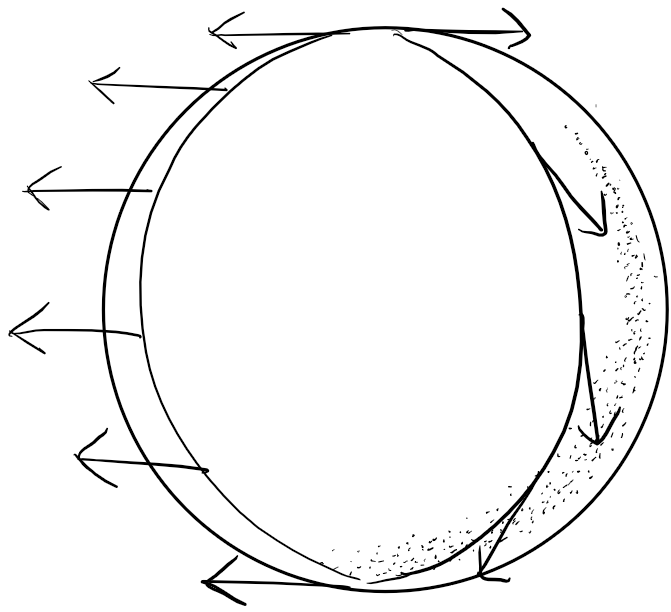
\includegraphics[width=0.3\textwidth]{parallel.png}
\end{center}
How much the vector is rotated is measured by the holonomy. The {\bf holonomy} $H\left( \gamma, A \right)$ on a $G$-bundle along a path $\gamma(t)$ is the group element in $G$ that maps the vector at the initial time to the vector at the final time. Writing out \eqref{parallel transport}
\begin{align}\label{parallel transport eq}
\partial_{\gamma'} u^{\mu} + A_{\gamma'} u &= 0 \nonumber \\
\gamma'(t) \left( \partial_{\gamma'} u^{\mu} + A_{\gamma'} u \right) &= 0 \nonumber \\
\frac{du(t)}{dt} + \gamma'(t) A_{\gamma'} u &= 0.
\end{align}
Since $A(t) \equiv \gamma'(t) A_{\gamma'} $ at different time may not commute, the solution to this is
\begin{align}
u(t) &= P\exp \left[-\int_0^t d\tau A(\tau) \right] u(0),
\end{align}
where $P$ signifies the path-ordered exponential
\begin{align}
P\exp \left[-\int_0^t A(\tau) d\tau \right] &= \sum_{n=0}^{\infty} \frac{(-1)^n}{n!} P \left[ \int_0^t d\tau A(\tau) \right]^n,
\end{align}
or more compactly,
\begin{align}
u(t) = Pe^{\int d\gamma \cdot A(t)} u(0).
\end{align}
So $Pe^{\int d\gamma \cdot A(t)}$ is the holonomy. (Recall that $A$ takes value in the Lie algebra of $G$, so the holonomy is indeed the group element.)


Suppose that $u(t)$ is the solution to \eqref{parallel transport eq} above. Under a local gauge transformation $g(\gamma(t))$,
\begin{align*}
\frac{d\tilde{u}}{dt} \equiv \frac{d}{dt} (gu)  
	&= \frac{d g(\gamma(t))}{dt}u + g \frac{du(t)}{dt} \\
    &= \gamma'(t) (\partial_{\gamma'} g) u - \gamma'(t) g A_{\gamma'} u, 
\end{align*}
where we have used the original parallel transport equation in the last line.
\begin{align*}
\frac{d\tilde{u}}{dt} &= \gamma'(t) \left( (\partial_{\gamma'} g) g^{-1} - g A_{\gamma'} g^{-1} \right) \tilde{u} \\
	&= -\left( g (\partial_{\gamma'} g^{-1}) + g A_{\gamma'} g^{-1} \right) \tilde{u} \\
    &= -\gamma'(t) \tilde{A}_{\gamma'} u \\
    &= - \tilde{A}(t) \tilde{u},
\end{align*}
where $\tilde{A}$ is the gauged transformed connection. The relation
\begin{align*}
H(\gamma, A') g(\gamma(0)) u(0) &= g(t) u(t) = g(\gamma(t)) H(\gamma, A) u(0)
\end{align*}
implies that the new holonomy is
\begin{align}
\boxed{H(\gamma, A') = g(\gamma(t)) H(\gamma, A) g^{-1}(\gamma(0))}.
\end{align}
The {\bf Wilson loop} is defined to be the trace of the holonomy of a loop $\gamma$, that is when $\gamma(t)=\gamma(0)$.
\begin{align}
\boxed{W(\gamma,A) = \Tr [H(\gamma,A)] = \Tr \left[ Pe^{\oint d\gamma \cdot A(t)} \right]}
\end{align}
Crucially, it is gauge invariant because the trace is invariant under conjugation by the same $g$.

%-------------------
\subsection{Example: Fractional statistics}
%-------------------

So far our discussion has mostly been about the \emph{classical} Chern-Simons theories. As with other gauge theories, the quantization of the Chern-Simons theories is done in the path integral formulation, which is outside the scope of this article. What is more, there is some subtlety in the calculation of the Wilson loop. So we will have to accept a few facts in order to move forward.

For simplicity, we will consider $U(1)$ quantum Chern-Simons theories. In this case, the Chern-Simons form reduces to
\begin{align}
A \wedge dA &= A_j \partial_k A_l dx^j \wedge dx^k \wedge dx^l
\end{align}
Since the group is abelian, there is no need for the path ordering in the Wilson loop anymore, and while we are at it, let us change the convention so that the phase has the same form as the Aharonov-Bohm phase in the natural units $\hbar = 1$.
\begin{align}\label{physicist wilson loop}
W(\gamma,A) = e^{iq\oint_{\gamma'} d\gamma \cdot A}. 
\end{align}
The vacuum expected value of a Wilson loop can be expressed in the path integral formulation as
\begin{align}
\langle W(\gamma) \rangle  
	&= \frac{ \bra{0} W(\gamma) \ket{0} }{ \braket{0|0} }
	= \frac{\int DA W(\gamma,A) \exp \left( i\int_M A \wedge dA \right)}{\int DA \exp \left( i\int_M A \wedge dA \right)}, 
\end{align}
where $\ket{0}$ is the vacuum state and $DA$ is the "measure" over the space of gauge fields. The amazing mathematical fact is that this is proportional to a link invariant, the {\bf linking number} $L$ \cite{Pachos12}, when $\gamma$ is now allowed to be a collection of loops:
\begin{align}\label{link formula}
\langle W (\gamma) \rangle = \exp \left[ \frac{i \pi}{k} \sum_{j,l} q_j q_l L(\gamma_j,\gamma_l) \right],
\end{align}
Two loops are linked when one is wrapped around the other. 
\begin{figure}\label{winding}
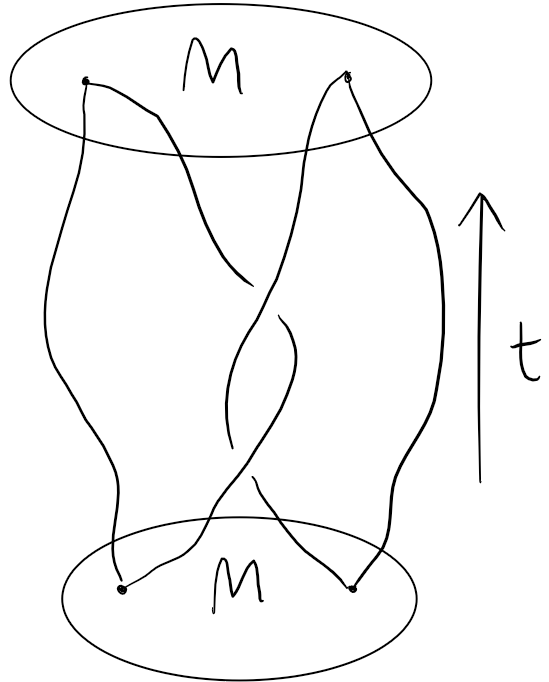
\includegraphics[width=0.25\textwidth]{linking.png}
\caption{Winding of the worldlines of two anyon-anti-anyon pairs. The worldlines can also be deformed into the process $T_2^{-1} T_1^{-1} T_2 T_1$ showing topological degeneracy in Section \ref{degeneracy}}
\end{figure}
A link in the Chern-Simons theory occurs in 2+1 dimensions. (A curve cannot be wrapped around another without intersecting in 2 dimensions.) That is, it is a linking of worldlines. Suppose that a counterclockwise braiding gives the linking number 1 (and a clockwise braiding gives -1). The vacuum expected value of the Wilson loop in Figure \ref{winding} will differ from that of a trivial Wilson loop $W(0)$ by
\begin{align}\label{anyon phase}
\langle W(\gamma) \rangle = \exp \left(\frac{2 i\pi q^2}{k} \right) \langle W(0) \rangle
\end{align}
This process can be interpreted as the creation of two pairs of {\bf anyons} and their antiparticles from the vacuum  followed by a $2\pi$ rotation of one particle around the other, and the annihilation into the vacuum again (because we are taking the vacuum expected value). 

However, there is clearly still a problem with the formula when $j=l$ because any curve intersects with itself at every point! This problem can be solved by the "framing" prescription. When considering the term $L(\gamma_j,\gamma_j)$, slightly displace $\gamma_j$. Call the displaced curve $\gamma_j'$, and replace $L(\gamma_j,\gamma_j)$ with $L(\gamma_j,\gamma_j')$. This prescription essentially creates a ribbon that can have a self-linking from a twist. (The twist has to be a full $2\pi$ rotation. No m{\"o}bius strip allowed!)
\begin{center}
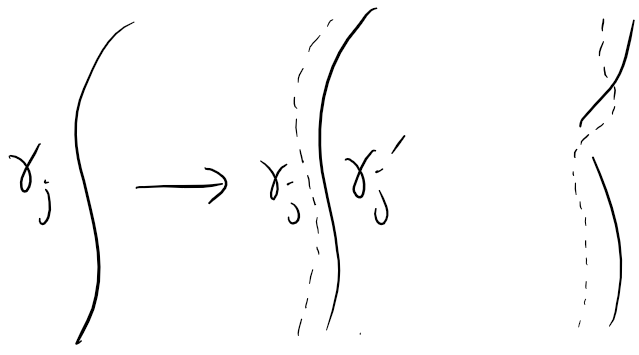
\includegraphics[width=0.3\textwidth]{ribbon.png}
\end{center}
Thus,
\begin{align}
\langle W(\gamma') \rangle = \exp \left( \frac{i\pi q^2}{k} L(\gamma,\gamma') \right) = e^{\frac{i\pi q^2}{k}} = e^{\frac{i\pi q^2}{k}} \langle W(0) \rangle. 
\end{align}
The additional phase from such a twist is $\theta = \pi q^2/k$. When interpreted as an anyon rotating about itself, this gives the anyon a spin $q^2/(2k)$ because $s = \theta/(2\pi)$. The Chern-Simons theories therefore demonstrate {\bf fractional statistics}.

%-------------------
\subsection{Example: Topological degeneracy}\label{degeneracy}
%-------------------

Suppose now that the spatial manifold is a torus. Processes that start in a vacuum state and end in a vacuum state commute with the Hamiltonian. Ones of these are unitary operators $T_1$ and $T_2$ that winds anyons around the torus along the meridian and the longitude respectively.
\begin{center}
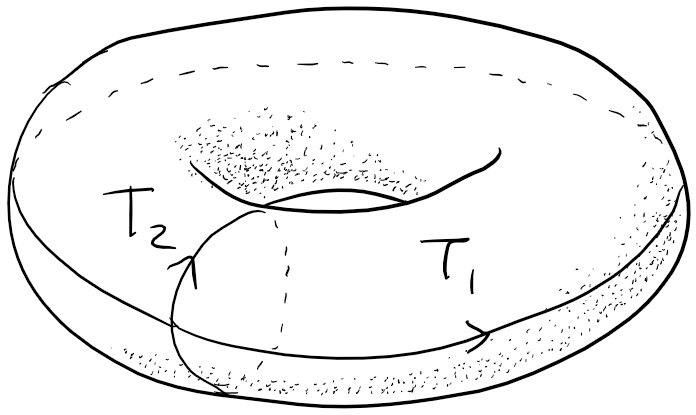
\includegraphics[width=0.35\textwidth]{torus.png}
\end{center}
The process $T_1^{-1}T_1$ or $T_2^{-1}T_2$ alone is a loop in spacetime that can be shrunk to a point. But interleaving them creates a link. More precisely, the worldlines of the process that creates an anyon-anti-anyon pair, apply $T_2^{-1} T_1^{-1} T_2 T_1$, and annihilate the pair can be deformed into the link in Figure \ref{winding}. So by \eqref{anyon phase},
\begin{align*}
T_2^{-1} T_1^{-1} T_2 T_1 = e^{2i\theta}
\end{align*}
or
\begin{align}
T_2 T_1 = e^{2i\theta} T_1 T_2.
\end{align}
Suppose that $|x \rangle$ is an eigenvector of $T_1$ with eigenvalue $e^{-ix}$.
\begin{align*}
T_1 (T_2 \ket{x}) &= e^{-2i\theta} T_2 T_1 \ket{x} \\
	&= e^{-i (x + 2\theta)} (T_2 \ket{x})
\end{align*}
So $T_2 \ket{x}$ is also an eigenvector of $T_1$ with eigenvalue $e^{-i (x + 2\theta)}$, which means that
\begin{align}
T_2 \ket{x} = \ket{x+2\theta}
\end{align}
If $\theta$ is a rational multiple of $\pi$: $\theta = \frac{\pi p}{r}$ with $p$ and $r$ that have no nontrivial common factor, then $\frac{2\pi p}{r}$ has at least $r$ distinct values: $0,1,2,\cdots r-1$. Since $T_1$ is unitary, all $q$ eigenvectors must be orthogonal. But $T_2$ is assumed to preserve the ground state, so the ground state must has degeneracy of at least $q$ purely from the topology of the manifold on which the Chern-Simons theory is defined.

This topological degeneracy is the essence of Kitaev's quantum memory \cite{Preskill}. Quantum information encoded in distinct degenerate ground states do not mix up because a random local perturbation is unlikely to send an anyon around the torus completely. Going further, some but not all non-abelian Chern-Simons theories even enable topologically protected universal quantum computation by anyon braiding. This makes sense since braiding of non-abelian anyons gives not just phases but unitary operations. However, not all set of unitary operations are universal. It has been found that anyon braiding in $SU(2)$ Chern-Simons theories at every level $k$ except $k=1,2,4$ allow for universal quantum computation \cite{Pachos12}. It is a marvel that one of the most exotic quantum field theories might potentially become a resource for engineering in the future!

\begin{thebibliography}{99}

\bibitem{Witten89}
Edward Witten, \emph{Quantum field theory and the Jones polynomial}, \href{http://link.springer.com/article/10.1007/BF01217730}{Communication in Mathematical Physics {\bf 121} 351 (1989)}.

\bibitem{Chern74}
Shiing-Shen Chern and James Harris Simons, \emph{Characteristic forms and geometric invariants}, \href{https://www.jstor.org/stable/1971013}{Annals of Mathematics
Second Series {\bf 99} 48 (1974)}.

\bibitem{Baez94}
John Baez and Javier P. Muniain, \emph{Gauge Fields, Knots, and Gravity}, World Scientific (1994).

%\bibitem{Deser82}
%S. Deser, R. Jackiw and S. Templeton, \emph{Three-Dimensional Massive Gauge Theories}, \href{https://doi.org/10.1103/PhysRevLett.48.975}{Physics Review Letters {\bf 48} 975 (1982)}.

\bibitem{Pachos12}
Jiannis K. Pachos, "Chern-Simons quantum field theories" in \emph{Introduction to Topological Quantum Computation}, Cambridge University Press (2012).

\bibitem{Preskill}
John Preskill, "Lecture Notes for Physics 229: Quantum Information and Computation" \href{http://www.theory.caltech.edu/ preskill/ph229}{www.theory.caltech.edu/ preskill/ph229}

%\bibitem{Kitaev03}
%Alexei Y. Kitaev, \emph{Fault-tolerant quantum computation by anyons}, \href{http://dx.doi.org/10.1016/S0003-4916(02)00018-0}{Annal of Physics {\bf 303} 2 (2003)}.

\end{thebibliography}

\appendix

%-------------------
\section{Exterior derivatives in 3 dimensions}\label{appendix}
%-------------------

The exterior derivative of a 0-form $F$ is the gradient.
\begin{align}
dF = F_x dx + F_y dy + F_z dz 
\end{align}
The exterior derivative of a 1-form $\omega = A dx + B dy + C dz$ is
\begin{align*}
d\omega &= d (A dx + B dy + C dz) \\
	&= (A_x dx + A_y dy + A_z dz) \wedge dx \\
    & + (B_x dx + B_y dy + B_z dz) \wedge dy \\
    & + (C_x dx + C_y dy + C_z dz) \wedge dz \\
    &= - A_x dx \wedge dy + A_z dz \wedge dx \\
    & + B_x dx \wedge dy - B_z dy \wedge dz \\
    & - C_x dz \wedge dx + C_y dy \wedge dz \\ 
    &= (C_y-B_z) dy \wedge dz + (A_z - C_x) dz \wedge dx + (B_x - A_y) dx \wedge dy.
\end{align*}
This returns the definition of the curl if we map the 2-forms to their complementary 1-forms. We can do this because $\Lambda V^1 = V$ and $\Lambda V^2$ in 3 dimensions are isomorphic as vector spaces, so we could pretend that every 2-form is a vector! \footnote{The map that realizes this pretension is the Hodge star operator or Hodge dual, which relies on a metric.}

The exterior derivative of a 2-form $\omega = A dy \wedge dz + B dz \wedge dx + C dx \wedge dy$ is
\begin{align*}
d\omega &= d(A dy \wedge dz + B dz \wedge dx + C dx \wedge dy) \\
	&= (A_x dx + A_y dy + A_z dz) \wedge dy \wedge dz \\
    &+ (B_x dx + B_y dy + B_z dz) \wedge dz \wedge dx \\
    &+ (C_x dx + C_y dy + C_z dz) \wedge dx \wedge dy \\
    &= (A_x + B_y + C_z) dx \wedge dy \wedge dz.
\end{align*}
Again, this is a 3-form. But $\Lambda^3 V$ is 1-dimensional, so this can be identified with the scalar $A_x + B_y + C_z$ and hence the divergence.

The identity $d(d\omega) = 0$ then translates to
\begin{align*}
\nabla \times (\nabla f) &= 0, \\
\nabla \cdot (\nabla \times A) &= 0.
\end{align*}

\end{document}